\documentclass[frenchb,16pt,parskip=half-]{scrartcl}
\usepackage[utf8]{inputenc}\usepackage[T1]{fontenc}
\usepackage[top=1cm,bottom=1cm,margin=1cm]{geometry}
\usepackage{lmodern,xspace,multicol,url,graphicx,babel}
\urlstyle{sf}\pagestyle{empty}
\begin{document}
\begin{minipage}[b]{4cm}
	 \centering
    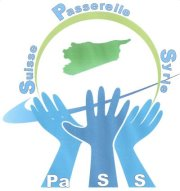
\includegraphics[width=\linewidth]{img/logopass.jpg}\\
	 {\tiny \url{suissesyrie@gmail.com}}
\end{minipage}\hfill
\begin{minipage}[b]{11cm}\centering\Large
    En lien avec l'association PASS\\
     le CO du Belluard soutient les\\ victimes du conflit en Syrie%\\[1em]~ 
\end{minipage}\hfill
\begin{minipage}[b]{4cm}
	 \centering
    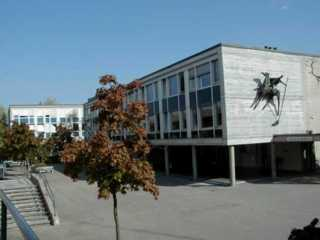
\includegraphics[width=\linewidth]{img/logobellu.png}
	 {\tiny \url{www.co-belluard.ch}}
\end{minipage}%\vfill
\begin{center}
\end{center}\vspace{-2em}
\begin{minipage}[c]{5cm}
    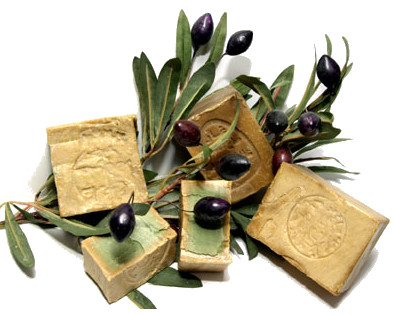
\includegraphics[width=\linewidth]{img/sav04.jpg}
\end{minipage}\hfill
\begin{minipage}[c]{8.5cm}\centering\huge
   par la vente de\\ \sc{savons d'Alep}\\ 7.-- pièce
\end{minipage}\hfill
\begin{minipage}[c]{5cm}
    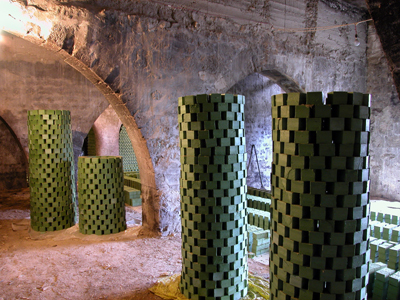
\includegraphics[width=\linewidth]{img/sav03.jpg}
\end{minipage}\vfill
Fabriqué depuis 4000 ans,
    le savon d'Alep a été le premier savon créé par les hommes! Entièrement naturel,
    son procédé de fabrication et sa composition n'ont jamais varié depuis l'Antiquité.
\vfill
Le savon d'Alep est un produit naturel, qui ne contient aucun:\\[-1.8em]
\begin{multicols}{3}
    \begin{itemize}
        \item colorant
        \item conservateur
        \item graisse animale
        \item produit de synthèse
        \item solvant
        \item fixateur de parfum
    \end{itemize}
\end{multicols}%\vfill
Ancêtre du savon de Marseille, le savon d'Alep s'utilise également comme:
\begin{itemize}
    \item Shampooing: 1 à 2 fois par semaine
    \item Masque du visage: laisser agir 1 minute puis rincer à l'eau  claire
    \item Mousse à raser
    \item Nettoyant pour le linge délicat
    \item Antimites: mettre un morceau de savon dans l'armoire pour protéger le linge
\end{itemize}\vfill
\begin{center}
    Le bénéfice de la vente des savons d'Alep sera entièrement versé à l'association \emph{PASS},
    qui aide entres autres les déplacés et les victimes de la guerre en Syrie.

    \vfill
    {\huge Un grand merci pour votre soutien!}
\end{center}
\vfill
\begin{minipage}[t]{.38\linewidth}
    PASS,\\ Route Joseph-Chaley 35\\ 1700 Fribourg\\ 079 766 99 41
\end{minipage}
\begin{minipage}[t]{.6\linewidth}
    ~\\ \url{suissesyrie@gmail.com}\\ \url{https://www.facebook.com/PasserelleSuisseSyrie}\\ CCP: 12-689870-3
\end{minipage}
\end{document}
